\documentclass[]{article}
\usepackage{lmodern}
\usepackage{amssymb,amsmath}
\usepackage{ifxetex,ifluatex}
\usepackage{fixltx2e} % provides \textsubscript
\ifnum 0\ifxetex 1\fi\ifluatex 1\fi=0 % if pdftex
  \usepackage[T1]{fontenc}
  \usepackage[utf8]{inputenc}
\else % if luatex or xelatex
  \ifxetex
    \usepackage{mathspec}
  \else
    \usepackage{fontspec}
  \fi
  \defaultfontfeatures{Ligatures=TeX,Scale=MatchLowercase}
\fi
% use upquote if available, for straight quotes in verbatim environments
\IfFileExists{upquote.sty}{\usepackage{upquote}}{}
% use microtype if available
\IfFileExists{microtype.sty}{%
\usepackage{microtype}
\UseMicrotypeSet[protrusion]{basicmath} % disable protrusion for tt fonts
}{}
\usepackage[unicode=true]{hyperref}
\hypersetup{
            pdfborder={0 0 0},
            breaklinks=true}
\urlstyle{same}  % don't use monospace font for urls
\usepackage[]{biblatex}
\addbibresource{../../Bibliography/Dissertation.bib}
\usepackage{graphicx,grffile}
\makeatletter
\def\maxwidth{\ifdim\Gin@nat@width>\linewidth\linewidth\else\Gin@nat@width\fi}
\def\maxheight{\ifdim\Gin@nat@height>\textheight\textheight\else\Gin@nat@height\fi}
\makeatother
% Scale images if necessary, so that they will not overflow the page
% margins by default, and it is still possible to overwrite the defaults
% using explicit options in \includegraphics[width, height, ...]{}
\setkeys{Gin}{width=\maxwidth,height=\maxheight,keepaspectratio}
\IfFileExists{parskip.sty}{%
\usepackage{parskip}
}{% else
\setlength{\parindent}{0pt}
\setlength{\parskip}{6pt plus 2pt minus 1pt}
}
\setlength{\emergencystretch}{3em}  % prevent overfull lines
\providecommand{\tightlist}{%
  \setlength{\itemsep}{0pt}\setlength{\parskip}{0pt}}
\setcounter{secnumdepth}{0}
% Redefines (sub)paragraphs to behave more like sections
\ifx\paragraph\undefined\else
\let\oldparagraph\paragraph
\renewcommand{\paragraph}[1]{\oldparagraph{#1}\mbox{}}
\fi
\ifx\subparagraph\undefined\else
\let\oldsubparagraph\subparagraph
\renewcommand{\subparagraph}[1]{\oldsubparagraph{#1}\mbox{}}
\fi

% set default figure placement to htbp
\makeatletter
\def\fps@figure{htbp}
\makeatother


\date{}

\begin{document}

\section{Result}\label{result}

\subsection{Usage overview}\label{usage-overview}

Over the week, teams created 1805 entities and 1529 relationships in
total. The number of entities teams created ranged from 24 to 223 (M=82,
SD=39.9), and the number of relationships ranged from 7 to 237 (M=69.5,
SD=51.0). The large variety of modeled data was related to team
strategy, which will be detailed later.

Overview of the survey items indicates that students rated positive on
CAnalytics overall, as shown in Figure \autocite{fig:survey}. CAnalytics
were ranked favorably in all aspects except cognitive load. They had a
close to neutral feeling towards cognitive load, which suggests that the
task is still cognitive heavy.

\begin{figure}
\centering
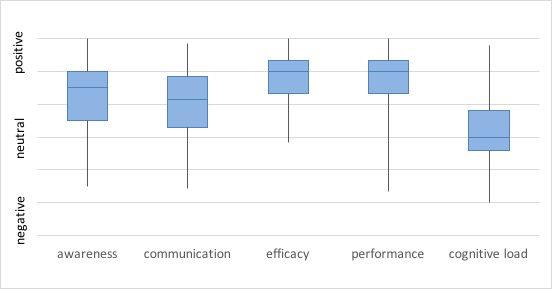
\includegraphics{./survey/survey_boxchart.jpg}
\caption{Survey responses (box shows Q1-Q3 and median; whiskers show
maximum and minimum)}\label{fig:survey}
\end{figure}

\subsection{Behavior of data modeling and data
analysis}\label{behavior-of-data-modeling-and-data-analysis}

We examined the pattern of data modeling and data analysis by looking at
a visualization of the entire interaction log (e.g.~Figure
\autocite{fig:sequence} shows the interaction log of one team). Teams
started with data modeling as they got themselves familiar with the
documents. However, teams did not wait to start analysis till they
finished data modeling; instead, the activity of data modeling and data
analysis were highly intertwined after certain point. Participants
switched from one activity to the other activity frequently. The state
transition diagram \autocite{fig:transition} better demonstrates the
transition between states, in which we encode the number of switches as
width of the link.

\begin{figure}
\centering
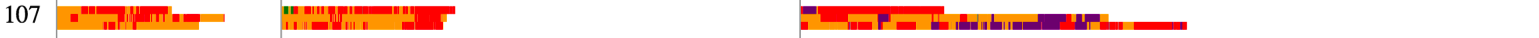
\includegraphics{./Log_analysis/action_sequence_vis/G107.png}
\caption{Visualization of interaction logs of Team 107. Each row of
colored marks indicates the sequence of top level activities a
participant performed.}\label{fig:sequence}
\end{figure}

\begin{figure}
\centering
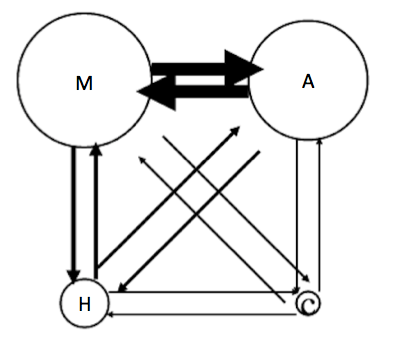
\includegraphics{./Log_analysis/state_transition/activity_transition-G107.png}
\caption{State transition diagram of interaction logs of Team 107. Each
node is an activity, whose size represents the time spent on the it; a
link represents a switch from one activity to another, whose width
encodes the number of switches.}\label{fig:transition}
\end{figure}

\begin{figure}
\centering
\includegraphics{./artifact_analysis/exemplar_artifacts.jpg}
\caption{User created network graphs. a) Exemplar network with filtering
strategy; b) network with accretion strategy; c) network consisting of
separate clusters; d) network consisting of connected
clusters}\label{fig:network}
\end{figure}

To look at the consequence of intertwined data modeling and data
analysis, we examined the analytic product teams created, the network
graph in particular because social relationships played the most
critical role in this specific scenario and teams spent most time on
network analysis (as reflected from the log). We found the network views
fell into one of two categories: the networks consisted of 1) separate
clusters, or 2) connected clusters. For example, networks from 8 teams
(36\%, mean performance=7.8) consist of separate clusters (Figure
\autocite{fig:network}b). Nodes within a cluster are connected,
representing information space of a robbery case; Nodes between clusters
are nonetheless not connected, indicating each robbery is a
self-contained case. However, these teams still claimed connections
between robberies in their report. Where did they externalize these
connections? Or did the teams simply share orally and held them in mind?
It turns out that teams documented possible relationships between
robberies in the notepad tool.

In contrast, 6 other teams (27\%, mean performance=8.3) created networks
composed of connected clusters. While a cluster is still a
representation of a robbery, some of them are connected through an
evidence node. An example is Figure \autocite{fig:network}c, in which we
mark four \emph{connectors} that link the clusters. These connectors
were key evidence that led the teams to hypothesize that those robberies
were related and might be committed by the same criminal group.

While many causes might account for the different network views, we
attempt to interpret the difference from a perspective of uncertainty.
For instance, links within a cluster are factual relationships literally
modeled from raw documents (e.g.~a white van was witnessed at a
location), but links between clusters are often inferences beyond
literally documented (e.g.~a white van at location A is the same van
witnessed at location B). Teams creating separate clusters only
represented facts in the network and held evidence with uncertainty in a
separate artifact. One advantage of distinguishing facts and inferences
is that teams can be aware of assumptions made when making a hypothesis.
And since all inferences are held in one place, teams are forced to
confront them and review their uncertainty iteratively in the process.
However, the strategy also adds difficulty to analysis as analysts may
overlook or fail to combine evidence scattered in different artifacts.

On the contrary, some other teams overlaid facts and inferences in the
same artifact. Both facts and inferences drove the layout of the
network, thus influencing team's framing of the problem. Most teams made
evaluation of the uncertainty of inferences when adding them to the
network. This strategy was relatively more interactive among teammates:
they needed to negotiate, evaluate, and reach consensus on the value and
validity of every inference. To some extent teams might forget whether a
relationship is factual or inferred, and ask whether conclusion derived
from the visualization can be trusted under uncertainty.

From granularity of entities, We noted a distinction between accretion
and filtering strategies in data modeling, similar to what we observed
in the paper prototype study. Filtering is selectively modeling of data
and adding to an artifact. Users must decide what information is
relevant, and thus what is to be excluded, as well as what granularity
of information is to model. Filtering requires more team coordination,
because teammates must reach a common ground of the current problem as
well as information needed to answer the problem. Figure
\autocite{fig:network}a is an example of filtering, highlighting only
the key information of each robbery and how robberies are connected.

Accretion is an attempt to comprehensively represent the problem by
adding all information to an artifact. Users extract every fact from the
document, regardless of its immediate relevance to the problem.
Accretion costs less coordination as it is relatively mechanical note
taking. A disadvantage of accretion is that it could be time consuming
to model all details and the produced artifact could be fairly complex.
An example is Team 108, who modeled every step the suspects took, which
resulted in many more entities than the average and much more cluttered
network view (Figure \autocite{fig:network}d). Users reported that they
spent too much time in details that they lost the bigger picture:

\begin{quote}
We would find ourselves glued to our computer screens, and spent too
much time on intelligence gathering rather than analysis (User 135)
\end{quote}

Different from the result in paper prototype study, however,
participants seemed to be more tempted to accretively add information
with CAnalytics. Students reflected that many annotations did not help
them solve the problem at all because those entities were unrelated to
their problem.

\begin{quote}
I felt that after we were done annotating, we hadn't really accomplished
anything and that we were no closer to solving the case than when we had
started. In the end it didn't really help that we had annotated the
data,
\end{quote}

Why did this happen? We guess both the context of classroom study and
the system design contributed. Unlike in the lab study where teams were
temporarily assembled, teams in a class evaluated peers either
consciously or unconsciously. Such social pressure motivated individuals
to make contributions, and to make \emph{visible} contributions more
than valuable contributions. The awareness features in our system
unfortunately made some contributions more \emph{visible} than others.
For example, creating an annotation would be immediately broadcast to
the team, whereas writing a hypotheses on a notepad produced no
notification, although the text was also shared. The selective awareness
seemed to also exert bias to recognition of contribution.

\subsection{Collaboration and
awareness}\label{collaboration-and-awareness}

Participants rated positively of the collaborative support. Participants
compared CAnalytics with state-of-the-art tools such as Analyst's
Notebook and PARC ACH. They liked the awareness features built on top of
the analytic capabilities and described it as \emph{``an analysts
notebook that multiple people could work on at once\ldots{}{[}and{]} an
analysts version of a Google Doc.''}

Participants reported that they could easily integrate team efforts.

\begin{quote}
they {[}teammates{]} were able to work directly off something that I had
also created. \textbf{This ability to work off of each other's own work
allowed us to all contribute to each element of the analytic process}.
An example of this would be when I was creating an association chart for
one of the bank robberies. I was able to cover my bases and include in
the chart all the information that I thought was relevant. At a later
time, one of my group members received the document of the same bank
robbery and found information he thought should be included in the
association chart that I had not included. \textbf{He was able to work
off of my initial diagram and add and manipulate it in order to include
additional relevant information I had missed}. (U31)
\end{quote}

The awareness features were received well. In the survey 88\% of the
students rated positively on their group awareness. When asked what
features helped them stay aware of team activities, 28 participants
mentioned the tool coordinator, 24 mentioned the notification system, 19
mentioned the history tool, 14 mentioned the real-time update of
user-generated data, 12 mentioned the collaborative editor, and 7
mentioned the message tool. While the number of mentions does not simply
indicate tool usefulness, it suggests users appropriate these features
and were explicitly aware of their support.

We categorized students' feedback based on the element of awareness, or
the essential problem of awareness of \emph{what}
\autocite{Schmidt2002}, into social awareness, information awareness,
action awareness, history awareness, and intention awareness, as shown
in Table \autocite{tab:awareness}.

\begin{figure}
\centering
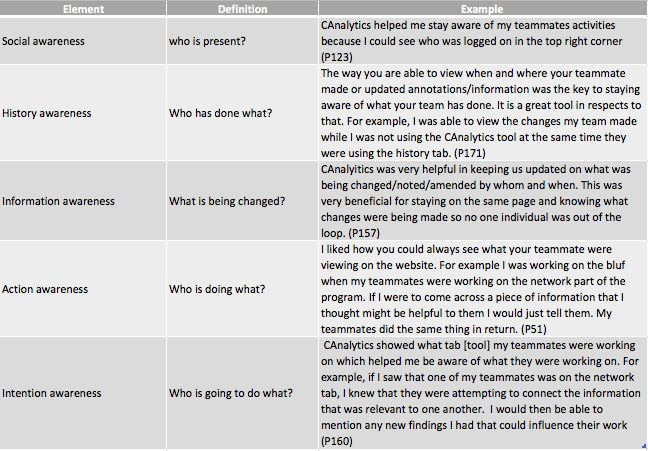
\includegraphics{./questionnaire/awareness.png}
\caption{Awareness aspects reported by
participants}\label{tab:awareness}
\end{figure}

By analyzing the interaction, we also found indicators of high
awareness. For example, we measured the number of entities accessed by
collaborators versus by the author only, and the time lapse when the
entity was first accessed by collaborator since created. While data
generated by users is automatically shared, it is up to collaborators to
choose to read the shared information or ignore information altogether.
A high awareness team would keep updated with collaborators' generated
information and read information soon after it is shared; whereas a low
awareness team might experience a significant delay or even never access
it. We found that most teams shared a high proportion of entities
(mean=77.6\%). We found that in average, 77.6\% of the created entities
were accessed by at least one teammate.

Students reported enjoying the use of CAnalytics. Specifically, being
able to see teammates contributing simultaneously that being aware that
teammates were contributing motivated themselves to contribute.

\begin{quote}
the notifications every time you saw someone annotated something kept
you peace at mind that your teammates are also working efficiently on
this project. (U64)
\end{quote}

\begin{quote}
During class I wasn't sure if my teammates were doing work for that
class or another thing but then seeing their dot {[}tool indicator{]}
switch between applications on the software and updates pop up on my
screen I knew they were doing work for 231. (U141)
\end{quote}

\begin{quote}
The fact that you can see what other teammates are doing and they can
see what you are doing creates a sense of accountability in terms of
separating the work load. (User 51)
\end{quote}

One major critique is the lack of sharing of intermediate analytic
insight for close collaboration. When individuals are exploring
visualizations (e.g.~zoom, filter, pan, drag, highlight), an insight
pops up with a specific visualization state. Students complaint that
they could not easily communicate that insight together with the
associate views to the team. The team could ``be looking at the same
information but arranged in completely different ways'' (P131). Unable
to share immediate insights in the graphic context seems to make
communication out of context.

\printbibliography

\end{document}
